\documentclass[xcolor=dvipsnames]{beamer}
\makeatletter\def\Hy@xspace@end{}\makeatother
\usepackage{graphicx, color, amssymb, amsmath, bm, rotating, graphics,
epsfig, multicol, amsthm, animate}
\usepackage{media9}
\usepackage[english]{babel}
\usepackage[T1]{fontenc}
\usepackage[ansinew]{inputenc}
\usepackage[authoryear]{natbib}
%\newcommand{\newblock}{}  %needed to make beamer and natbib play nice
\usepackage{tikz, caption}
% A counter, since TikZ is not clever enough (yet) to handle
% arbitrary angle systems.
\newcount\mycount

\usetheme{Boadilla}
%\usecolortheme{lily}
\definecolor{MUgold}{RGB}{241,184,45}
\usecolortheme[named=MUgold]{structure}
\setbeamercolor{structure}{bg=Black}
\setbeamercolor{structure}{fg=MUgold}
\setbeamercolor{title}{bg=Black}
\setbeamercolor{frametitle}{bg=Black, fg=MUgold}
\setbeamercolor{title in head/foot}{fg=Black, bg=MUgold}
\setbeamercolor{author in head/foot}{fg=MUgold, bg=Black}
\setbeamercolor{institute in head/foot}{fg=MUgold, bg=Black}
\setbeamercolor{date in head/foot}{fg=MUgold, bg=Black}
\setbeamercolor{item projected}{bg=MUgold, fg=Black}
\usesubitemizeitemtemplate{\tiny\raise1.5pt\hbox{\color{Black}$\blacktriangleright$}}
\setbeamercovered{transparent=0}
\beamertemplatenavigationsymbolsempty

\title[AT-PSO for Spatial Design]{Adaptively Tuned Particle Swarm Optimization for Spatial Design}

%\subtitle{}
\author[Matt Simpson]{Matthew Simpson}
\institute[Mizzou Stat / SAS]{Department of Statistics, University of Missouri\\
                              SAS Institute, Inc.}
\date{August 3, 2016}

\begin{document}

\begin{frame}
\titlepage
\centering
{\scriptsize
Joint work with Christopher Wikle and Scott H. Holan\\~\\
Research supported by the NSF-Census Research Network}
\end{frame}

\begin{frame}
\frametitle{Overview of the Talk}
\begin{columns}
\begin{column}{0.5\textwidth}
\begin{enumerate}
\item What is particle swarm optimization (PSO)?\\
 \citep*{blum2008swarm, clerc2010particle, clerc2011spso}\\~\\
\item New adaptively-tuned PSO algorithms.\\~\\
\item Using (adaptively-tuned) PSO for spatial design.\\~\\
\item Example adding locations to an existing monitoring network.
\end{enumerate}
\end{column}
\begin{column}{0.5\textwidth}
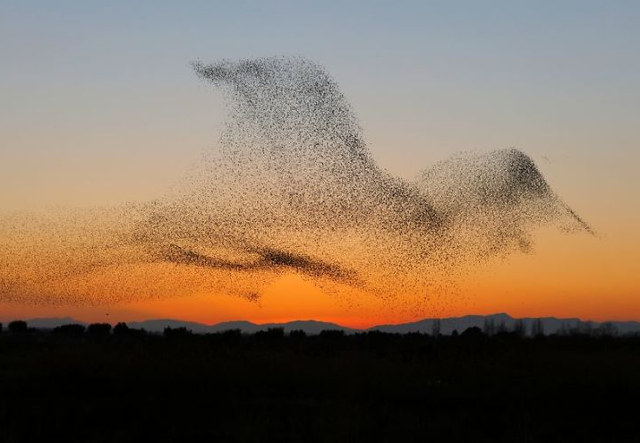
\includegraphics[width = 0.99\textwidth]{birds3.jpg}
\end{column}
\end{columns}
\end{frame}

\begin{frame}
  \frametitle{Particle Swarm Optimization --- Intuition}
Put a ``swarm'' of particles in the search space:\\
\begin{itemize}
\item[] Don't search alone, pay attention to what your neighbors are doing!
\end{itemize}
\begin{center}
\includemedia[
  width=0.9\textwidth,
  activate=pageopen,
  addresource=fishschool.mp4,   %passcontext,  %show VPlayer's right-click menu
  flashvars={
    %important: same path as in `addresource'
    source=fishschool.mp4
    &autoPlay=true
    &loop=true
  }
]{\fbox{Click!}}{VPlayer.swf}
\end{center}
Best for {\color{red} complex} objective functions which are {\color{red} cheap} to compute, and when {\color{red} near-optimal} solutions are useful.
\end{frame}

\begin{frame}
\frametitle{Particle Swarm Optimization}
Goal: minimize some objective function $Q(\bm{\theta}): \mathbb{R}^D \to \mathbb{R}$.\\~\\
Populate $\mathbb{R}^D$ with $n$ particles. Define particle $i$ in period $k$ by:
\begin{itemize}
\item a {\color{red}location} \hfill $\bm{\theta}_i(k)\in \mathbb{R}^D$;\hspace{2.5cm}\phantom{.}
\item a {\color{red}velocity} \hfill $\bm{v}_i(k) \in \mathbb{R}^D$;\hspace{2.5cm}\phantom{.}
\item a {\color{red}personal best} location \hfill $\bm{p}_i(k) \in \mathbb{R}^D$;\hspace{2.5cm}\phantom{.}
\item a {\color{red}neighborhood (group) best} location \hfill $\bm{g}_i(k) \in \mathbb{R}^D$.\hspace{2.5cm}\phantom{.} \\~\\
\end{itemize}

\pause

Basic PSO: update particle $i$ from $k$ to $k+1$ via: \\
\begin{itemize}
\item  For $j=1,2,\dots,D$:
\begin{align*}
v_{ij}(k+1) &= {\color{blue}\omega} v_{ij}(k) +  \mathrm{U}(0,{\color{blue}\phi_1})\times\{p_{ij}(k) - \theta_{ij}(k)\} \\
     &\;\phantom{= \omega v_{ij}(k)}+  \mathrm{U}(0,{\color{blue}\phi_2})\times\{g_{ij}(k) - \theta_{ij}(k)\}\\
& = \mbox{{\color{red}inertia}} + \mbox{{\color{red}cognitive}} + \mbox{{\color{red}social}},\\
\theta_{ij}(k+1) &= \theta_{ij}(k) + v_{ij}(k+1),
\end{align*}
\item Then update personal and group best locations.
\end{itemize}
\end{frame}

\begin{frame}
\frametitle{PSO --- Parameters}
\begin{align*}
v_{ij}(k+1) &= {\color{blue}\omega} v_{ij}(k) +  \mathrm{U}(0,{\color{blue}\phi_1})\times\{p_{ij}(k) - \theta_{ij}(k)\} \\
     &\;\phantom{= \omega v_{ij}(k)}+  \mathrm{U}(0,{\color{blue}\phi_2})\times\{g_{ij}(k) - \theta_{ij}(k)\}
\end{align*}
{\color{blue}Inertia} parameter: ${\color{blue}\omega}$.
\begin{itemize}
\item Controls the particle's tendency to keep moving in the same direction.\\~\\
\end{itemize}

{\color{blue}Cognitive} correction factor: ${\color{blue}\phi_1}$.
\begin{itemize}
\item Controls the particle's tendency to move toward its personal best.\\~\\
\end{itemize}

{\color{blue}Social} correction factor: ${\color{blue}\phi_2}$.
\begin{itemize}
\item Controls the particle's tendency to move toward its group best.\\~\\
\end{itemize}

Default choices:
\begin{itemize}
\item $\omega = 0.7298$, $\phi_1 = \phi_2 = 1.496$ \citep*{clerc2002particle}.
\item $\omega = 1/(2\ln 2)\approx 0.721$, $\phi_1=\phi_2=1/2 + \ln 2\approx 1.193$ \citep*{clerc2006stagnation}.
\end{itemize}

\end{frame}

\begin{frame}
\frametitle{PSO --- Neighborhood Topologies}
Sometimes it is useful to restrict the flow of information across the swarm --- e.g. complicated objective functions with many local optima.\\~\\

Particles are only informed by their {\color{blue}neighbors} for their group best $\bm{g}_i(k)$.\\
\ \ $\to$ \emph{No matter where they are in the search space}. \\~\\

\pause

We use the stochastic star neighborhood topology \citep*{miranda2008stochastic}.\\
\begin{itemize}
\item Each particle informs itself and $m$ random particles.\\
$\to$ informants sampled with replacement once during initialization.
\item On average each particle is informed by $m$ particles.
\item A small number of particles will be informed by many particles.
\end{itemize}


\end{frame}

\begin{frame}
\frametitle{Many variants on basic PSO exist}
See e.g. \citet*{clerc2011spso}, \citet*[][appendix]{simpson2017adaptively}.
\begin{itemize}
\item Handling search space constraints.
\item Coordinate free velocity updates.
\item Parallelization.
\item Asynchronous updates.
\item Redraw neighborhoods.
\item Bare-bones PSO (BBPSO) --- no velocity term.
\end{itemize}
\end{frame}


\begin{frame}
\frametitle{Adaptively Tuning PSO}
In PSO larger $\omega$ $\implies$ more exploration, smaller $\omega$ $\implies$ more exploitation.\\~\\

\pause

Idea: deterministic inertia PSO (DI-PSO) \\
\ \ \ \ \ \ \ $\to$ slowly decrease $\omega(k)$ over time \citep*{eberhart2000comparing}.
\begin{itemize}
\item Hard to set appropriately for any given problem.\\~\\
\end{itemize}

\pause

AT-PSO: tune $\omega(k)$ using an analogy with adaptively tuned random walk Metropolis \citep*{andrieu2008tutorial}.\\~\\

Can also create AT-BBPSO algorithms.
\end{frame}


\begin{frame}
\frametitle{Adaptively Tuned PSO --- $\omega(k)$'s progression}
Define the improvement rate of the swarm in period $k$:
\begin{align*}
R(k) = &&  \mbox{proportion of particles that improved}\\
       &&  \mbox{on their personal best last period.}
\end{align*}
\pause
Let ${\color{blue}R^*}$ denote a target improvement rate, and\\
\ \ ${\color{blue}c}$ denote an adjustment factor.\\~

Update $\omega(k)$ via:
\begin{align*}
\log \omega(k+1) &= \log\omega(k) + {\color{blue}c}\{R(k+1) - {\color{blue}R^*}\}
\end{align*}

\pause

Defaults: ${\color{blue}R^*}\in[0.3, 0.5]$, ${\color{blue}c} = 0.1$.
\end{frame}

\begin{frame}
\frametitle{AT-PSO/AT-BBPSO Simulation Study Results}
Intuition: tuning $\omega(k)$ allows the swarm to adjust the exploration / exploitation tradeoff on the fly based on current swarm conditions.\\
\begin{itemize}
\item This has a tendency to speed up convergence.\\
\item ...but convergence may be premature in multi-modal problems.\\~\\
\end{itemize}

\pause

Overview of results from a simulation study:
\begin{itemize}
\item AT-PSO performs better than PSO on ``hard enough'' problems... 
\item ...but has trouble with many local optima.\pause
\item AT-BBPSO is often the best performing algorithm for complex, multimodal objective functions...
\item ...but is less competitive for easier objective functions.
\end{itemize}
\end{frame}

\begin{frame}
\frametitle{Spatial Design --- Problem Setup}
Goal: want to learn about the spatial field $Y(\bm{u})$, $\bm{u}\in\mathcal{D}\subset \mathbb{R}^2$. \pause\\~\\

We observe a noisy signal of $Y(\bm{u})$ at $N_s$ fixed monitoring locations, $\bm{s}_1, \dots, \bm{s}_{N_s}$,
and assume:
\begin{align*}
Z(\bm{u}) = Y(\bm{u}) + \varepsilon(\bm{u})
\end{align*}
for all $\bm{u}\in\mathcal{D}$, and $\varepsilon(\bm{u}) \stackrel{iid}{\sim} \mathrm{N}(0, \tau^2)$. \pause\\~\\

Assume $Y(\bm{u}) = \bm{x}(\bm{u})'\bm{\beta} + \delta(\bm{u})$ with
\begin{align*}
\delta(\bm{u}) \sim \mathrm{GP}(0, C_{\bm{\phi}}(\cdot, \cdot))
\end{align*}
where $\bm{x}(\bm{u})$ is a vector of covariates known at all locations $\bm{u}\in\mathcal{D}$. \pause \\~\\

Where should we put additional monitoring locations, $\bm{D} = \{\bm{d}_1, \dots, \bm{d}_{N_d}$\}?
\end{frame}

\begin{frame}
\frametitle{Spatial Design --- MSPE and Kriging}
Sensible goal: choose new locations to minimize MSPE. \\~\\

\pause

With $\tau^2$ and $\bm{\phi}$ known, universal kriging MSPE is {\footnotesize \citep*{cressie2011statistics}:}
{\footnotesize
\begin{align*}
& \sigma_{uk}^2(\bm{u};\bm{D}, \widehat{\bm{\theta}})=C_{\widehat{\bm{\phi}}}(\bm{u}, \bm{u}) - \bm{c}_Y(\bm{u};\bm{D})'\bm{C}_Z^{-1}(\bm{D})\bm{c}_Y(\bm{u};\bm{D}) \ + \\
& \left\{\bm{x}(\bm{u})  - \bm{X}'\bm{C}_Z^{-1}(\bm{D})\bm{c}_Y(\bm{u};\bm{D})\right\}'\left\{\bm{X}'\bm{C}_Z^{-1}(\bm{D})\bm{X}\right\}^{-1}\left\{\bm{x}(\bm{u})  - \bm{X}'\bm{C}_Z^{-1}(\bm{D})\bm{c}_Y(\bm{u};\bm{D})\right\}
\end{align*}
}
\pause
What about when $\tau^2$ and $\bm{\phi}$ are estimated? \pause\\~\\

Parameter uncertainty universal kriging MSPE:
\begin{align*}
\approx \sigma^2_{puk}(\bm{u};\bm{D},\widehat{\bm{\theta}}) = \sigma^2_{uk}(\bm{u};\bm{D},\widehat{\bm{\theta}}) + \mbox{ stuff, }
\end{align*}
depending on the FI matrix and gradient of predictor wrt $\bm{\theta}$\\
\citep*{zimmerman1992mean,abt1999estimating}.
\end{frame}

\begin{frame}
\frametitle{Spatial Design --- Design Criteria}
Ideal design criteria: choose design points to minimize...
\begin{itemize}
\item Mean/total MSPE: $\overline{Q}_{puk}(\bm{D}) = \int_{\mathcal{D}}\sigma_{puk}^2(\bm{u};\bm{D},\widehat{\bm{\theta}})d\bm{u}$
\item Maximum MSPE: $Q^*_{puk}(\bm{D}) = \max_{\bm{u}\in\mathcal{D}}\sigma_{puk}^2(\bm{u},\bm{D},\widehat{\bm{\theta}})$\\~\\
\end{itemize}

\pause

This is computationally infeasible. \\~\\

Realistic criteria: approximate with a grid of target points $\bm{r}_1,\dots,\bm{r}_{N_t}$:
\begin{itemize}
\item Minimize $\overline{Q}_{puk}(\bm{D}) = \sum_{i=1}^{N_t}\sigma_{puk}^2(\bm{r}_i;\bm{D},\widehat{\bm{\theta}})$
\item Minimize $Q_{puk}^*(\bm{D}) = \max_{i=1,2,\dots,N_t}\sigma_{puk}^2(\bm{r}_i;\bm{D},\widehat{\bm{\theta}})$
\end{itemize}

\end{frame}

\begin{frame}
  \frametitle{Optimzation for Spatial Design}
  The spatial design optimization problem cannot be solved in closed form. \\~\\ \pause

  Usual solution: grid up the space and use an exchange algorithm.\\
 \citep*{nychka1998design,wikle1999space,wikle2005dynamic} \\~\\ \pause

  In principle, \emph{any} location is a valid design point, not just the grid.\\
  $\implies$ why not use PSO? \pause Other points in its favor: \\
  \begin{itemize}
  \item Near-optimal solutions are nearly as valuable as optimal solutions.
  \item Objective function is cheap in universal kriging.
  \item More expensive in kriging with parameter uncertainty, but doable.
  \item Highly multi-modal objective function (e.g. switch two locations).\pause
  \end{itemize}

  Genetic algorithms also reasonable, e.g. \citet*{hamada2001finding}.
\end{frame}

\begin{frame}
  \frametitle{Example: Ozone Monitoring in Harris County, TX}
  \begin{columns}
    \begin{column}{0.6\textwidth}
      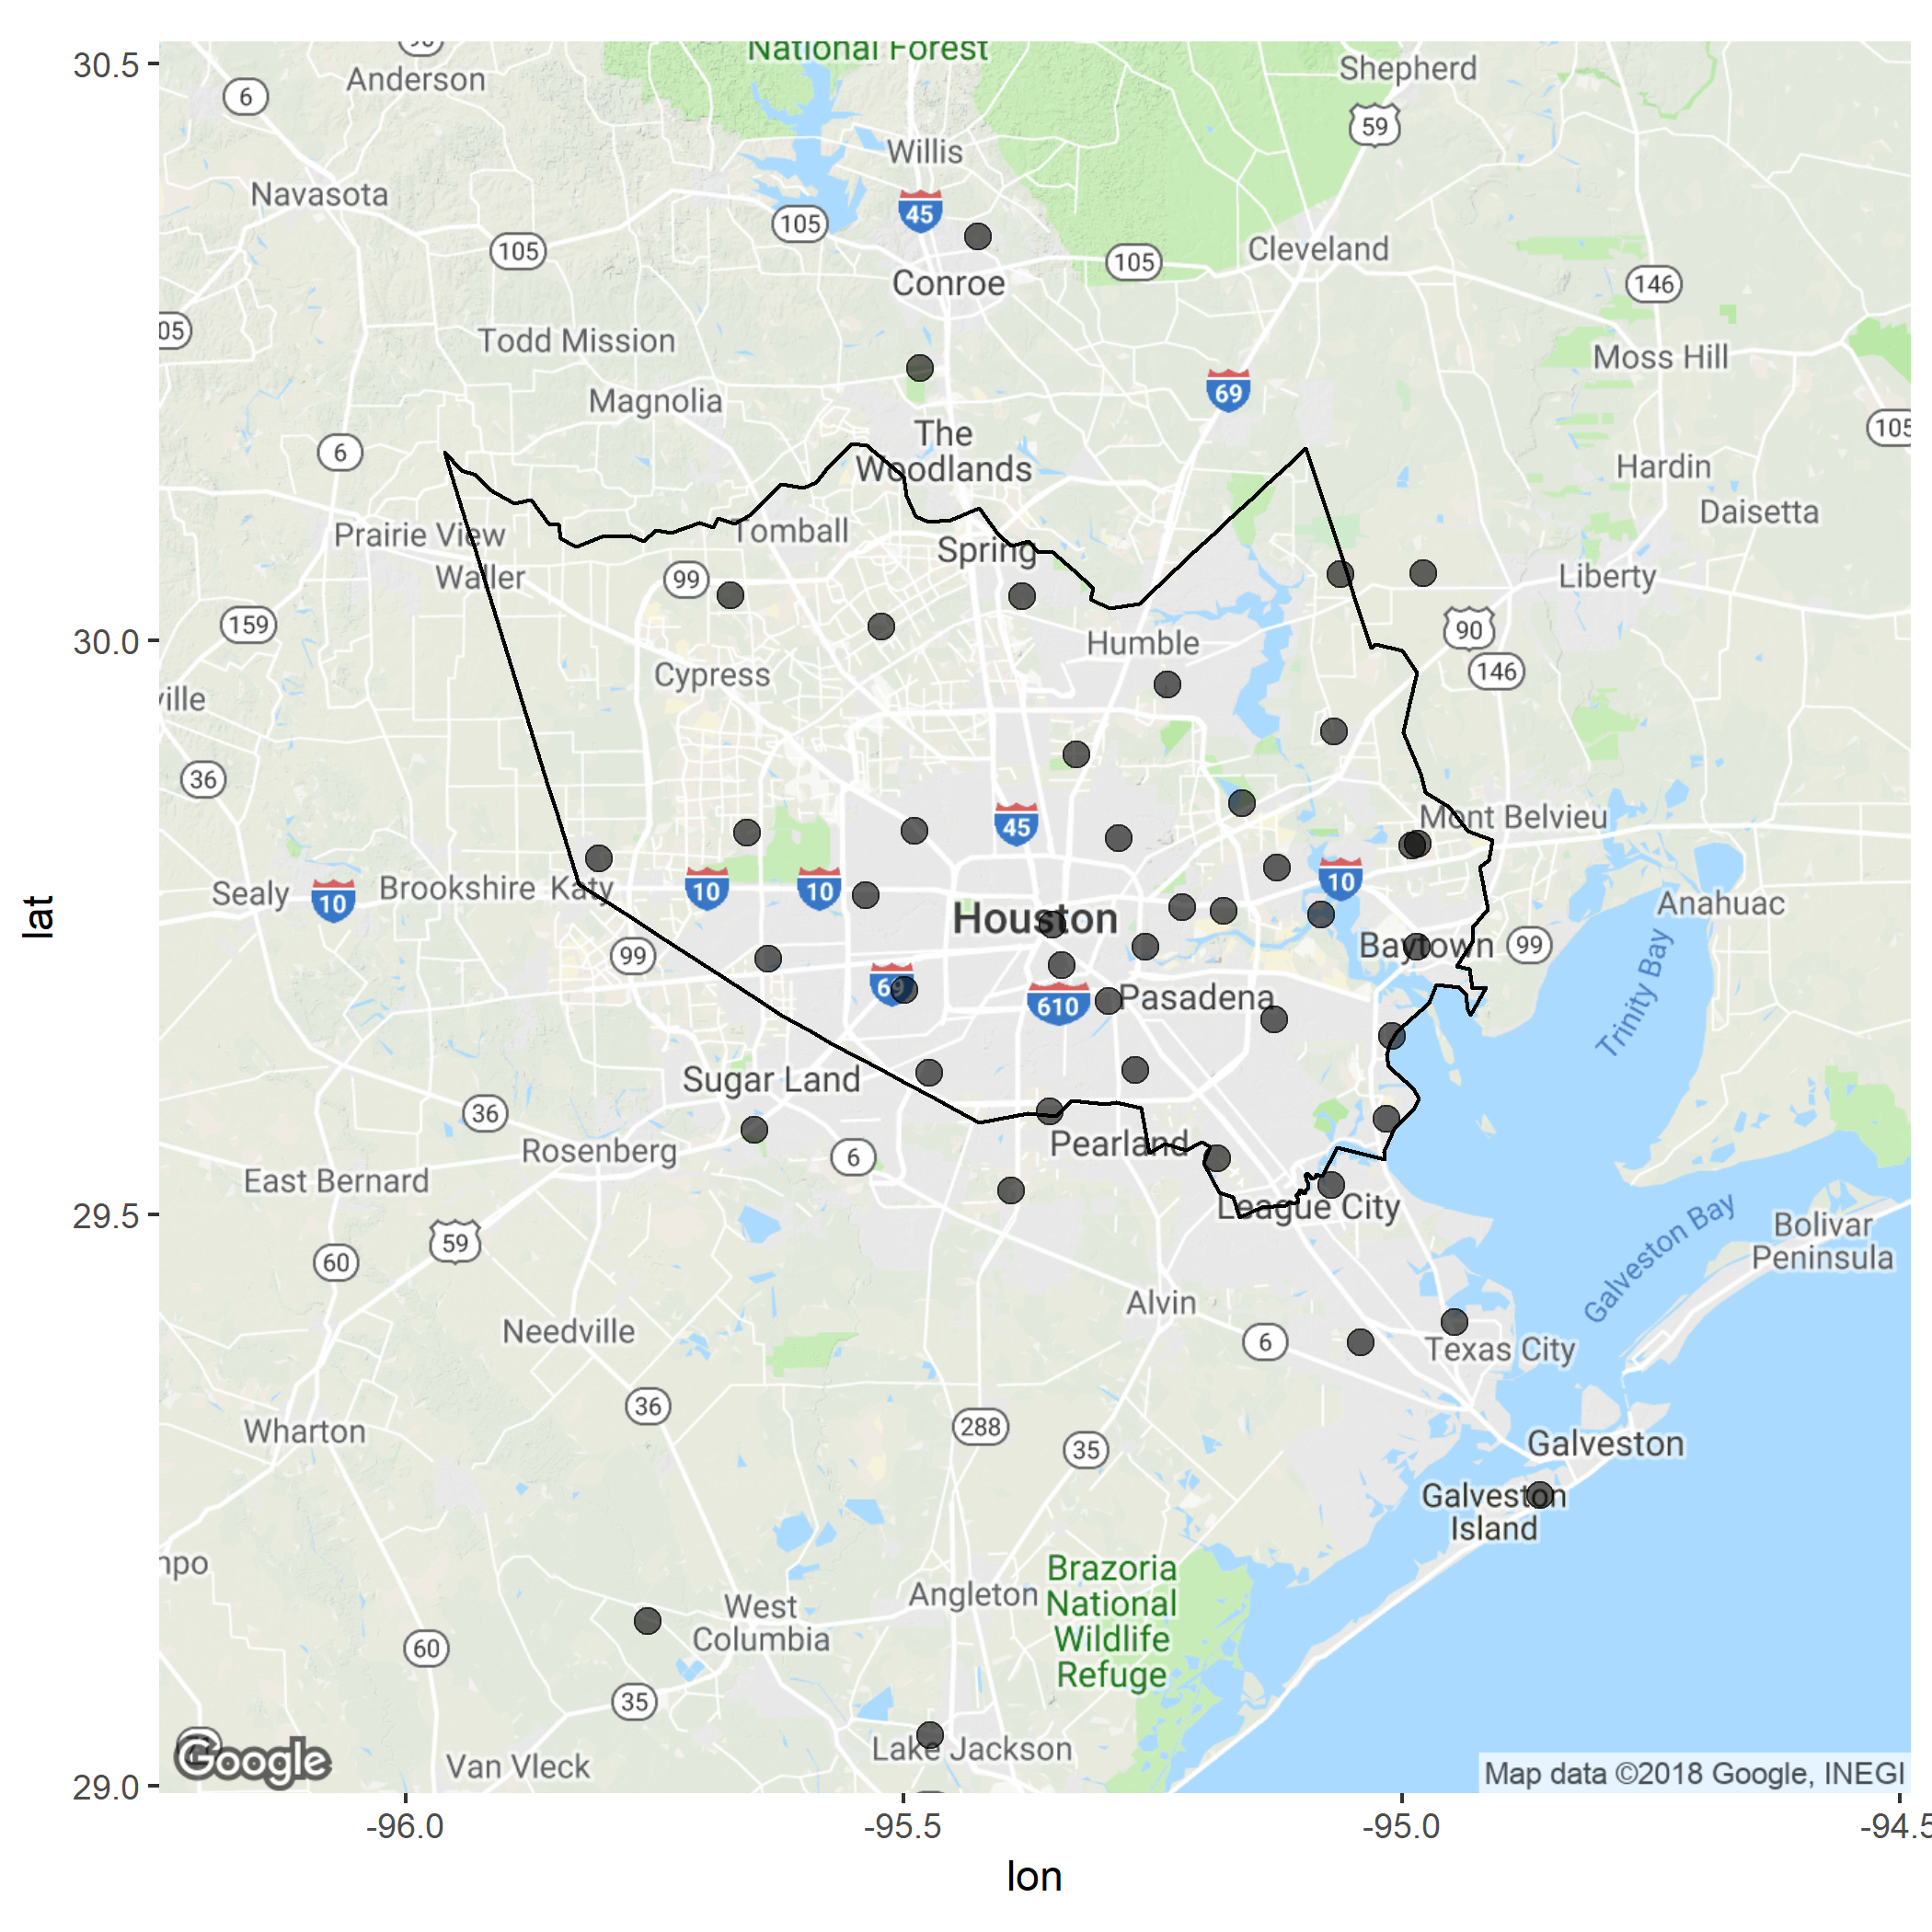
\includegraphics[width = 0.95\textwidth]{../code/kriging/houston.png}\\
      Map via ggmap \citep*{ggmap2013}.
    \end{column}
    \begin{column}{0.4\textwidth}
      \begin{itemize}
      \item Ozone concentration is associated with increased risk of cardiac arrest \citep*{ensor2013case}. \\~
      \item In August 2016, there were 44 active monitoring locations near Houston, TX. \\~
      \item Harris County, TX, contains 33 of these locations.
      \end{itemize}
    \end{column}
  \end{columns}
\end{frame}

\begin{frame}
  \frametitle{Hypothetical Design Problem and Data}
  Want to learn more about ozone concentrations in Harris County. \\~

  Where to put 100 new monitoring locations within the county? \\
  \begin{itemize}
  \item[] Note: nearby locations outside of the county still useful for estimation.\\~\\
  \end{itemize}\pause

  Data from the Texas Commission on Environmental Quality (TCEQ)
  \begin{itemize}
  \item Monitoring locations measure several air quality indicators.
  \item Ozone: daily maximum eight-hour ozone concentration (DM8) in parts per billion.\\
    $\to$ maximum of all contiguous 8-hour means for that day.
  \item Some locations have missing data.
  \end{itemize}
\end{frame}

\begin{frame}
  \frametitle{Model and Design Criteria}
  Model:
  \begin{itemize}
  \item Linear mean function in spatial coordinates: $\bm{x}(\bm{u})' = (u_1, u_2)$.
  \item Exponential covariance function:
    \begin{align*}
      C(\bm{u},\bm{v}) = \sigma^2\exp(-||\bm{u} - \bm{v}||/\psi)
    \end{align*}
  \item Estimate $(\bm{\theta}, \bm{\delta})$ via maximum likelihood. \\~\\ \pause
  \end{itemize}

  Design Criteria:
  \begin{itemize}
  \item Mean MSPE w/ parameter uncertainty $\overline{Q}_{puk}(\bm{d})$.
  \item Maximum MSPE w/ parameter uncertainty $Q^*_{puk}(\bm{d})$.
  \item Approximate each with a grid of 1229 points in Harris County.
  \end{itemize}
\end{frame}

\begin{frame}
  \begin{columns}
    \begin{column}{0.4\textwidth}
  \begin{scriptsize}
\begin{tabular}{lrr}
Algorithm & $\overline{Q}_{puk}$ & $Q^*_{puk}$ \\\hline
Uniform & 16.40 & 26.80 \\\hline
PSO1 & \bf{14.40} & \bf{20.63} \\
  PSO2 & 14.45 & \bf{21.03}\\
  PSO1-CF & 15.53 & 23.54 \\
  PSO2-CF & 15.77 & 23.16 \\
   \hline
AT1-PSO1 & \bf{14.38} & \bf{20.57} \\
  AT1-PSO2 & 14.56 & 23.18 \\
  AT1-PSO1-CF & 15.96 & 23.33 \\
  AT1-PSO2-CF & 15.60 & 24.02 \\
   \hline
AT2-PSO1 & \bf{14.42} & \bf{21.13} \\
  AT2-PSO2 & \bf{14.32} & 22.11 \\
  AT2-PSO1-CF & 15.85 & 24.00 \\
  AT2-PSO2-CF & 15.95 & 23.63 \\
   \hline
AT1-BBPSO & 14.53 & 22.28 \\
  AT1-BBPSOxp & 15.87 & 22.19 \\
  AT1-BBPSO-CF & 14.65 & 21.33 \\
  AT1-BBPSOxp-CF & 14.84 & 22.34 \\
   \hline
AT2-BBPSO & 14.65 & 23.49 \\
  AT2-BBPSOxp & 15.21 & 23.25 \\
  AT2-BBPSO-CF & 14.63 & 21.92\\
  AT2-BBPSOxp-CF & 14.52 & 22.76 \\
   \hline
GA-11 & \bf{14.40} & 21.19 \\
  GA-21 & 15.20 & 23.21 \\
  GA-12 & 14.45 & \bf{20.84} \\
  GA-22 & 15.26 & 22.61 \\
\hline
\end{tabular}
\end{scriptsize}
\end{column}
\begin{column}{0.55\textwidth}
  Results:
  \begin{itemize}
  \item Uniform: uniformly sample new \\
\hspace{1.42cm} monitoring locations.\\
GA: genetic algorithm.
\item Bolded: top 5 for that design criterion (column).\pause
\item Objective function is simple enough that robustness of AT-BBPSO variants is unnecessary.\pause
\item PSO and AT-PSO variants tend to be the best.
\item GAs are competitive. \pause
\item With significantly fewer monitoring locations, PSO variants are the best.
  \end{itemize}
\end{column}
\end{columns}
\end{frame}

\begin{frame}
\frametitle{Best designs found according to $\overline{Q}_{puk}$ (left) and $Q^*_{puk}$ (right)}
{\centering
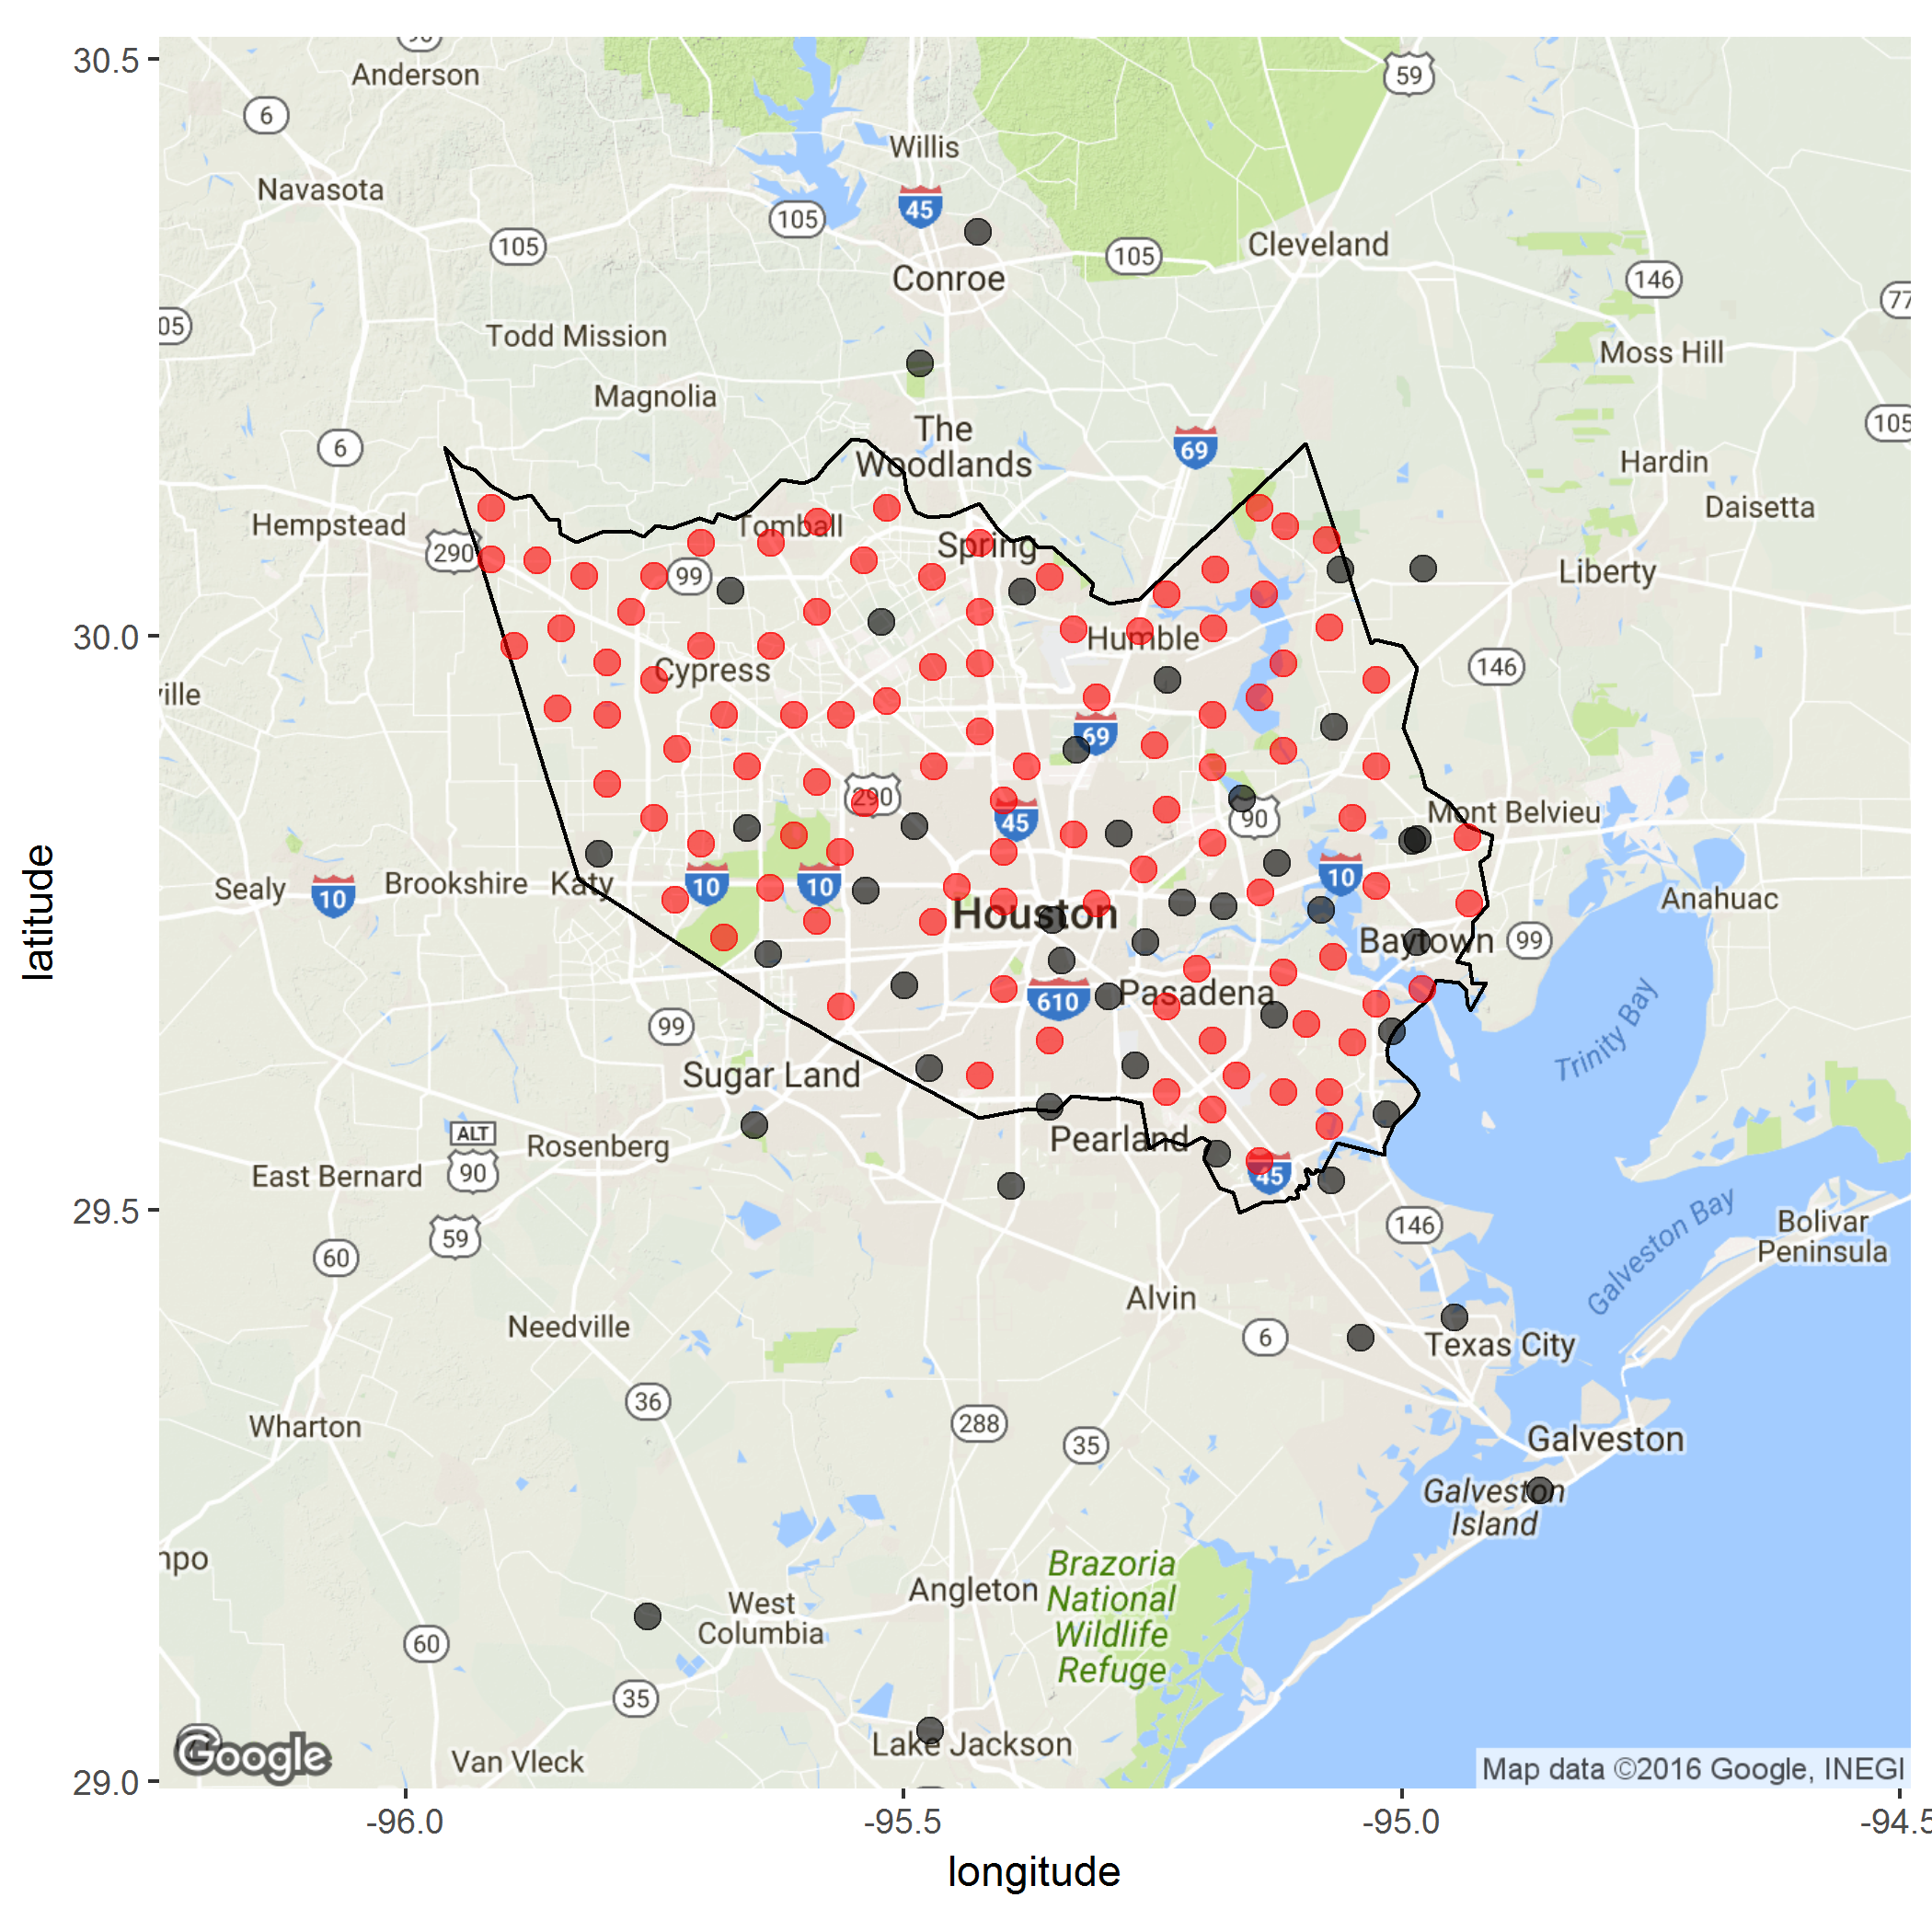
\includegraphics[width=.49\textwidth]{../doc/sig2pukmean.png}
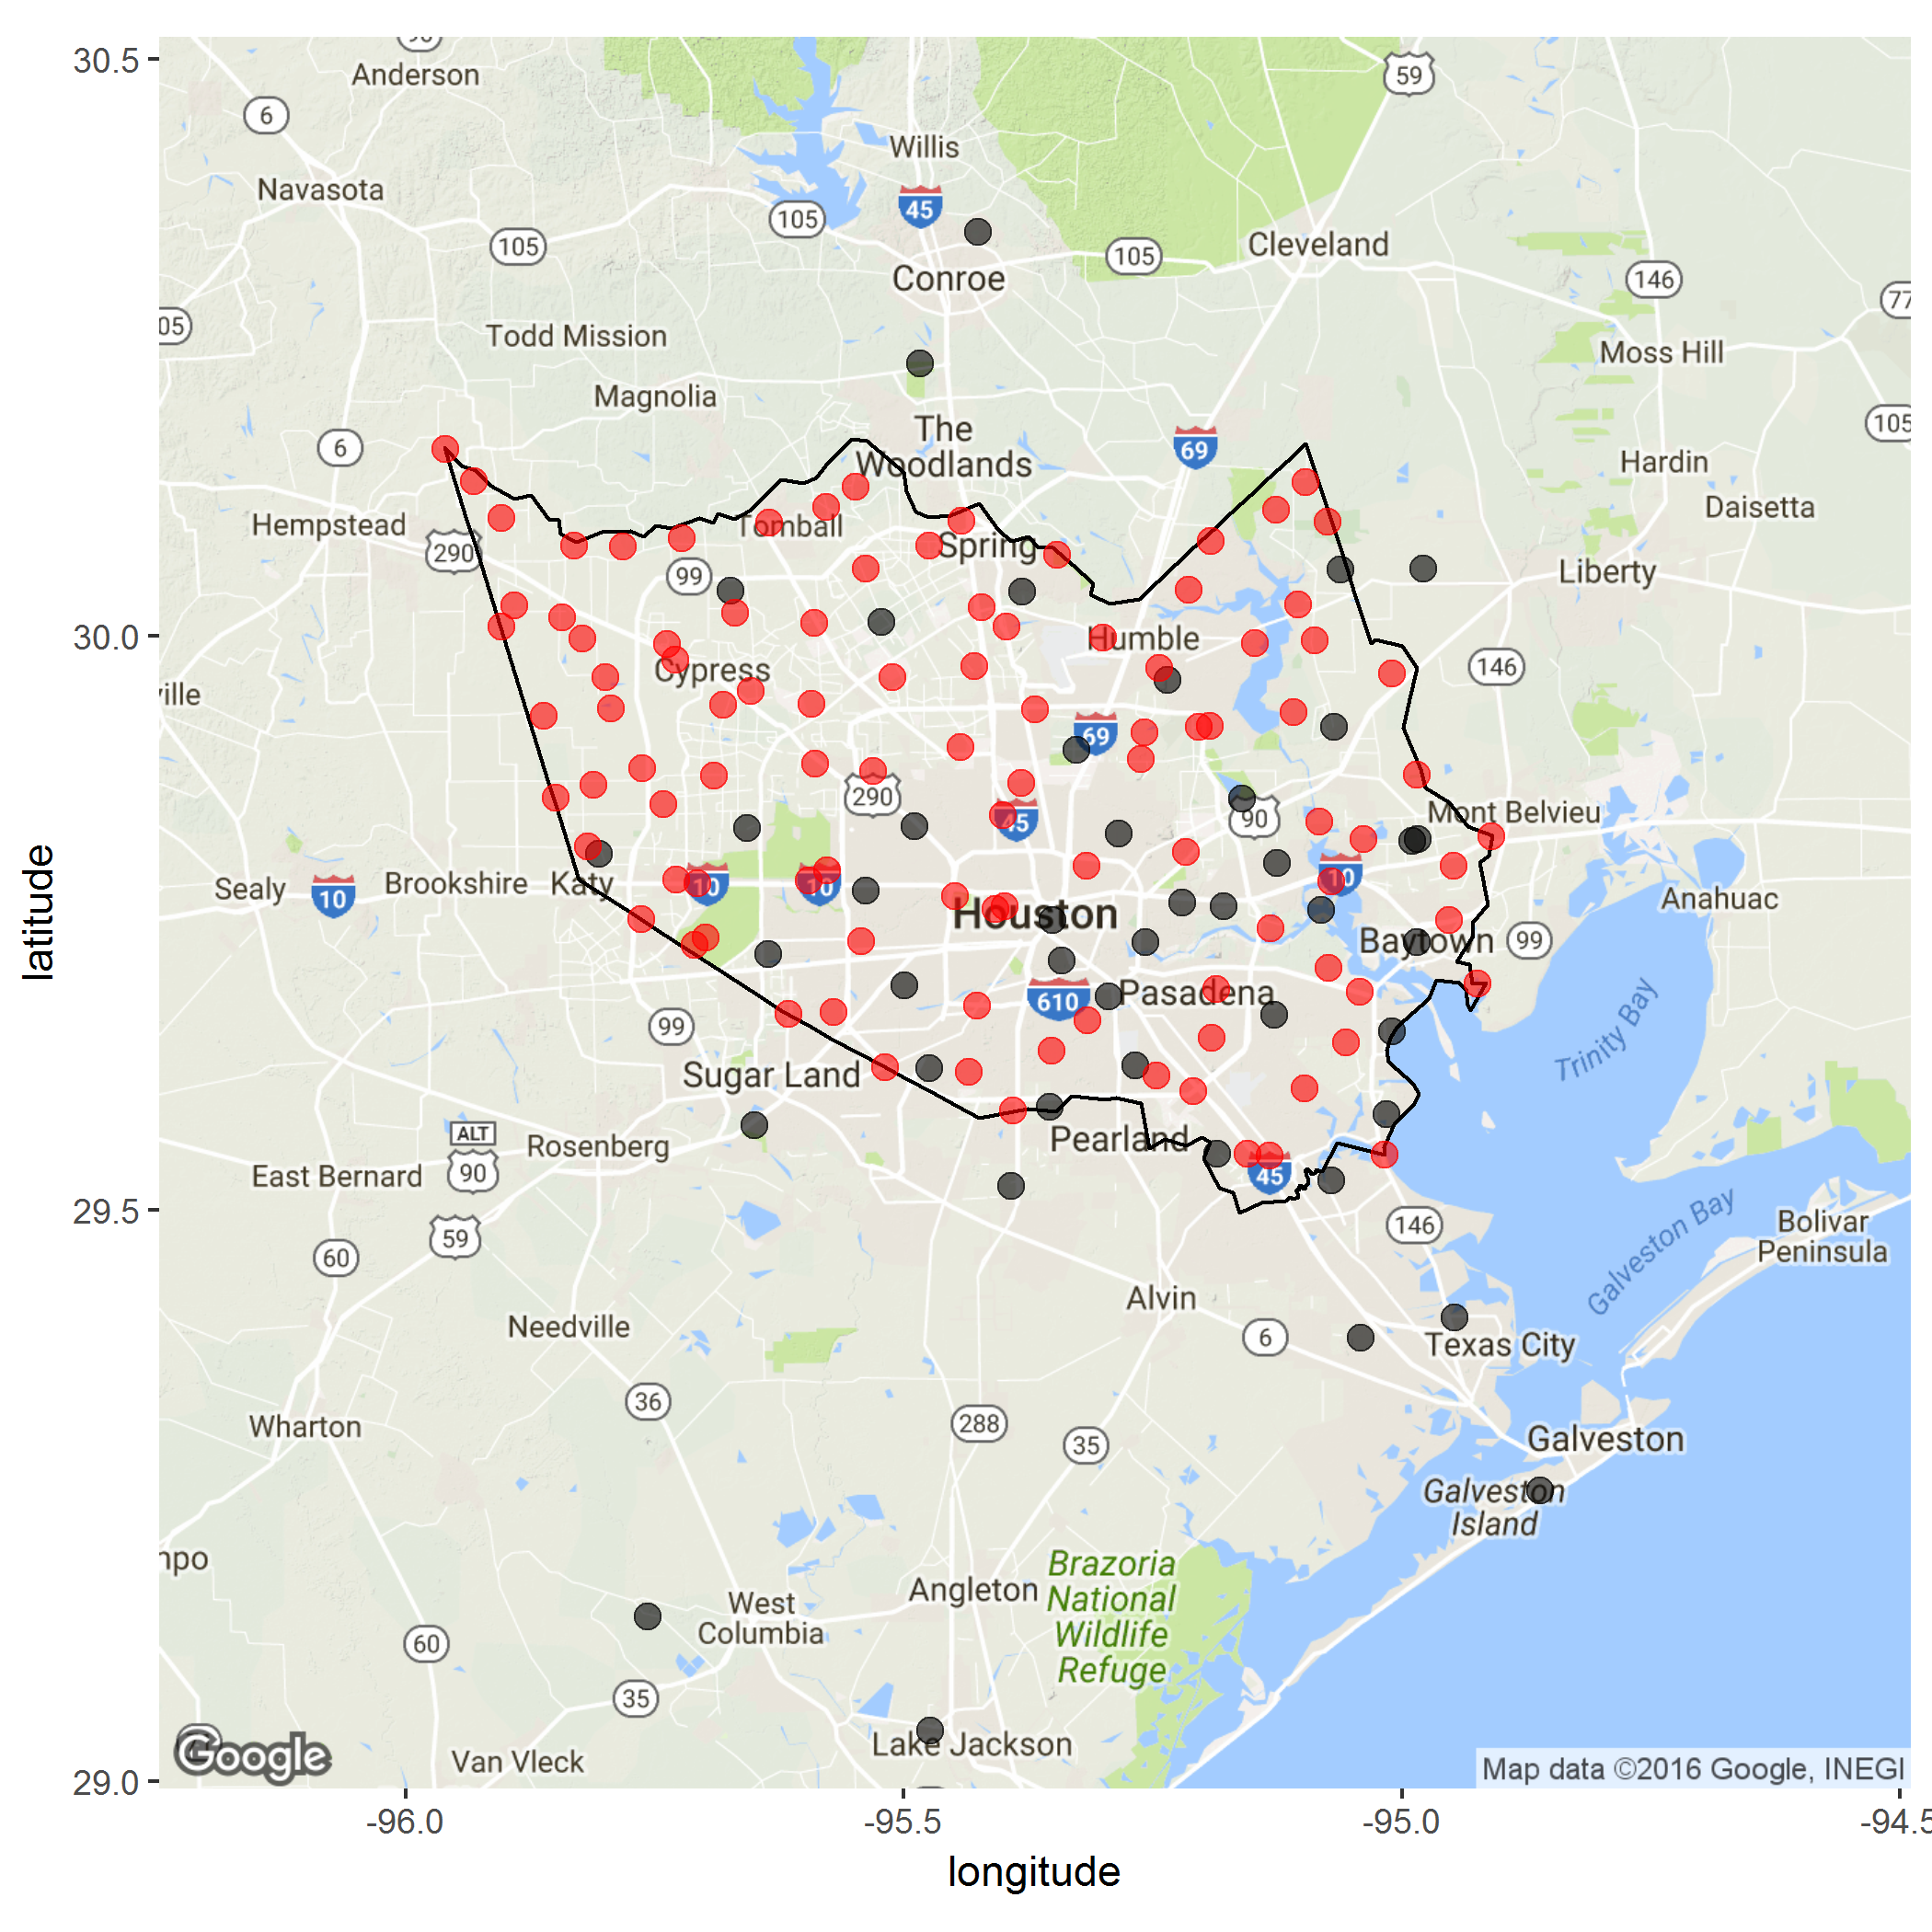
\includegraphics[width=.49\textwidth]{../doc/sig2pukmax.png}
}\\
Optimal design is highly dependent on the mean function\\ \citep*{zimmerman2006optimal}.\\~

Background map via ggmap \citep*{ggmap2013}.

\end{frame}

\begin{frame}
  \frametitle{Conclusions}
  \begin{itemize}
  \item Introduced new classes of adaptively tuned PSO and BBPSO algorithms.\\~\\ \pause
  \item AT-BBPSO performed well on very difficult problems --- quite robust to extreme multimodality. \\~\\ \pause
  \item AT-PSO performed well on difficult, but not too difficult problems. \\~\\ \pause
  \item For spatial design problems, standard PSO works well. \\~\\\pause
  \item For large enough spatial design problems, AT-PSO is attractive. \\~\\\pause
  \item Approach can easily be extended to spatio-\emph{temporal} design.
  \end{itemize}
\end{frame}

\appendix
\newcounter{finalframe}
\setcounter{finalframe}{\value{framenumber}}

\begin{frame}

      \begin{center}

        \font\endfont = cmss10 at 25.40mm
        \color{MUgold}
        \endfont
        \baselineskip 20.0mm

        Thank you!

      \end{center}


\end{frame}

\begin{frame}[allowframebreaks]
        \frametitle{References}
        \bibliographystyle{apalike}
        \bibliography{../doc/pso}
\end{frame}
\setcounter{framenumber}{\value{finalframe}}
\end{document}
